\begin{figure*}[h!]
    \centering
    \subfloat[Quenched (AR).]{%
        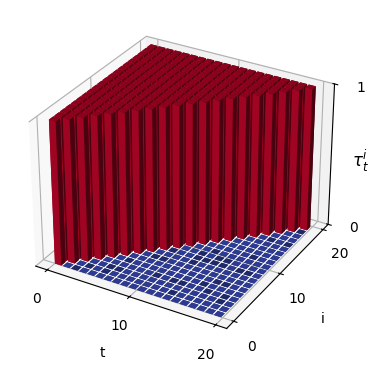
\includegraphics[width=0.23\textwidth]{figs/annealing_methods/Qwench.png}%
        \label{figure:tau:quenched}
    }
    \hfill
    \subfloat[Flat annealing.]{%
        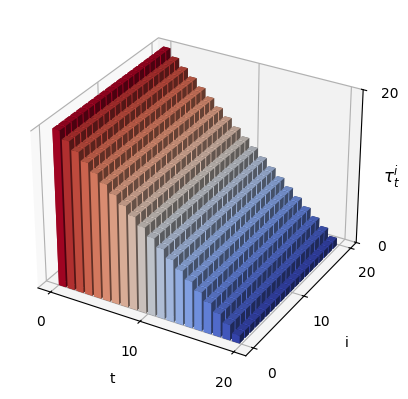
\includegraphics[width=0.23\textwidth]{figs/annealing_methods/Flat.png}%
        \label{figure:tau:flat}
    }
    \hfill
    \subfloat[Block annealing.]{%
        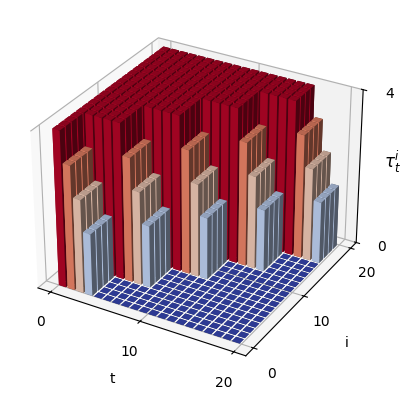
\includegraphics[width=0.23\textwidth]{figs/annealing_methods/Block.png}%
        \label{figure:tau:block}
    }
    \hfill
    \subfloat[Slide annealing.]{%
        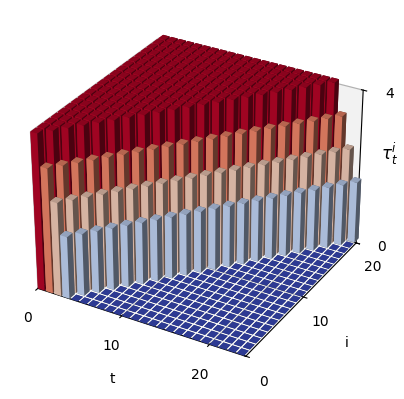
\includegraphics[width=0.23\textwidth]{figs/annealing_methods/Slide.png}%
        \label{figure:tau:slide}
    }

    \caption{We introduce $\boldsymbol{\tau}$-\emph{hyperschedules}, subjecting different token positions $i$ to different noise levels (red: high; blue: low) at different generation step $t$.
    %
    (a) Standard AR models (e.g., GPT) determine tokens one by one, ``quenching'' each of them to full determination in a single step, and can be seen as an extreme case of a diffusion model.
    (b) Standard diffusion models (e.g., SEDD) gradually anneal all tokens independently of position.
    (c) Block-wise annealing for blocks of width $\omega=4$.
    (d) Sliding window annealing (``smoothed'' AR) with window width $\omega=4$. These last two combine properties of both AR and diffusion.
    }
    \label{fig:four_subfigs}
\end{figure*}